% answers.tex —— 1977 年·甘肃卷 · 参考答案与详细解析片段
% 由 tools/generate_projects.py 依来源总账自 1977/1977_数学真题_甘肃_试题.md + 1977/1977_数学真题_甘肃_解析正文.md + 1977/1977_数学真题_甘肃_答案要点.md 生成，勿手改（改源 MD 后重跑）


\begin{gktip}
固定源为题面与解答连续排印的《试题解》扫描材料。下文逐题独立推导，并对照源解答复算关键结论：第 5 题源卷自注题意不清（注文全文引录于该题解析）；第 6 题源解答的代入行有漏字排印、且定高所用 $45^\circ$ 角未在题面给出；第 8(1) 题源卷导数记号印作 $\dfrac{dy}{dy}$——均按保留转录原则留注，最终结论与源一致。
\end{gktip}

\begin{answer}
\gksolhead{1}{}

\textbf{题目}：

用“$>$”、“$<$”、“$=$”号分别把下列各组数连接起来：

（1） $0.25+3\dfrac{1}{8}$ 与 $|-3.375|$；

（2） $\left(\dfrac{\sqrt{3}}{3}-\dfrac{1}{\sqrt{3}}\right)^{3}$ 与 $(-3)^{0}$；

（3） $-\lg 0.01$ 与 $\log_4\dfrac{1}{16}$；

（4） $\operatorname{tg} 44^\circ$ 与 $\operatorname{ctg} 44^\circ$。

\Needspace{4\baselineskip}
\textbf{解析}

\gksubpart{（1）}

\nopagebreak[4]
\[
0.25+3\frac{1}{8}=\frac{1}{4}+\frac{25}{8}=\frac{27}{8}=3.375,
\qquad
|-3.375|=3.375,
\]

故两数相等，用“$=$”号连接。

\gksubpart{（2）}

\Needspace{5\baselineskip}
由 $\dfrac{1}{\sqrt{3}}=\dfrac{\sqrt{3}}{3}$ 得

\nopagebreak[4]
\[
\left(\frac{\sqrt{3}}{3}-\frac{1}{\sqrt{3}}\right)^{3}=0,
\qquad
(-3)^{0}=1,
\]

故前者小于后者，用“$<$”号连接。

\gksubpart{（3）}

\nopagebreak[4]
\[
-\lg 0.01=-(-2)=2>0,
\qquad
\log_4\frac{1}{16}=\log_4 4^{-2}=-2<0,
\]

故 $-\lg 0.01>\log_4\dfrac{1}{16}$，用“$>$”号连接。

\gksubpart{（4）}

\Needspace{5\baselineskip}
$\operatorname{ctg}44^\circ=\tan(90^\circ-44^\circ)=\tan 46^\circ$。正切函数在 $(0^\circ,90^\circ)$ 上是增函数，且 $44^\circ<46^\circ$，故

\nopagebreak[4]
\[
\tan 44^\circ<\tan 46^\circ=\cot 44^\circ,
\]

用“$<$”号连接。

\gkanswer{答案（1）：$0.25+3\dfrac{1}{8}=|-3.375|$（用“$=$”号）。}

\gkanswer{答案（2）：$\left(\dfrac{\sqrt{3}}{3}-\dfrac{1}{\sqrt{3}}\right)^{3}<(-3)^{0}$（用“$<$”号）。}

\gkanswer{答案（3）：$-\lg 0.01>\log_4\dfrac{1}{16}$（用“$>$”号）。}

\gkanswer{答案（4）：$\operatorname{tg}44^\circ<\operatorname{ctg}44^\circ$（用“$<$”号）。}

\end{answer}
\begin{answer}
\gksolhead{2}{}

\textbf{题目}：

解答下列各题：

\Needspace{5\baselineskip}
（1） 计算：

\nopagebreak[4]
\[
\frac{2a}{a-3b}-\frac{6ab-24b^2}{a^2-7ab+12b^2}.
\]

\Needspace{5\baselineskip}
（2） 化简：

\nopagebreak[4]
\[
\frac{(a^{\frac{8}{5}}b^{-\frac{6}{5}})^{-\frac{1}{2}}\sqrt[5]{a^4}}{\sqrt[5]{b^3}}.
\]

\Needspace{5\baselineskip}
（3） 证明：

\nopagebreak[4]
\[
\frac{2\operatorname{ctg}x}{1+\operatorname{ctg}^2x}=\sin 2x.
\]

（4） 求函数 $y=\dfrac{1}{2}x^2+3x+9$ 的极值。

\Needspace{4\baselineskip}
\textbf{解析}

\gksubpart{（1）}

\Needspace{5\baselineskip}
在 $a\ne 3b$、$a\ne 4b$ 的条件下，

\nopagebreak[4]
\[
\frac{2a}{a-3b}-\frac{6ab-24b^{2}}{a^{2}-7ab+12b^{2}}
=\frac{2a}{a-3b}-\frac{6b(a-4b)}{(a-3b)(a-4b)}
=\frac{2a-6b}{a-3b}=2.
\]

\gksubpart{（2）}

\Needspace{5\baselineskip}
幂运算：$\left(a^{\frac{8}{5}}b^{-\frac{6}{5}}\right)^{-\frac{1}{2}}=a^{-\frac{4}{5}}b^{\frac{3}{5}}$，$\sqrt[5]{a^{4}}=a^{\frac{4}{5}}$，$\sqrt[5]{b^{3}}=b^{\frac{3}{5}}$，故

\nopagebreak[4]
\[
\frac{(a^{\frac{8}{5}}b^{-\frac{6}{5}})^{-\frac{1}{2}}\sqrt[5]{a^{4}}}{\sqrt[5]{b^{3}}}
=\frac{a^{-\frac{4}{5}}b^{\frac{3}{5}}\cdot a^{\frac{4}{5}}}{b^{\frac{3}{5}}}
=\frac{b^{\frac{3}{5}}}{b^{\frac{3}{5}}}=1.
\]

\gksubpart{（3）}

\Needspace{5\baselineskip}
在 $\sin x\ne 0$ 的条件下，由 $1+\operatorname{ctg}^{2}x=\csc^{2}x=\dfrac{1}{\sin^{2}x}$，

\nopagebreak[4]
\[
\frac{2\cot x}{1+\cot^{2}x}
=2\cot x\cdot\sin^{2}x
=2\cdot\frac{\cos x}{\sin x}\cdot\sin^{2}x
=2\sin x\cos x
=\sin 2x.
\]

\begin{gktip}
\textbf{源注}：源解答中间步骤把 $1+\operatorname{ctg}^{2}x$ 写作 $\sec^{2}x$（应为 $\csc^{2}x$），随后的「$2\operatorname{ctg}x\cos^{2}x$」一步与结论不相衔接；本库按 $\csc^{2}x$ 推证，最终结论与源一致。
\end{gktip}

\gksubpart{（4）}

\Needspace{5\baselineskip}
配方：

\nopagebreak[4]
\[
y=\frac{1}{2}x^{2}+3x+9=\frac{1}{2}(x+3)^{2}+\frac{9}{2}.
\]

抛物线开口向上，故当 $x=-3$ 时，$y$ 有极小值 $\dfrac{9}{2}$。

\gkanswer{答案（1）：$2$。}

\gkanswer{答案（2）：$1$。}

\gkanswer{答案（3）：见解析版}

\gkanswer{答案（4）：当 $x=-3$ 时，$y$ 有极小值 $\dfrac{9}{2}$。}

\end{answer}
\begin{answer}
\gksolhead{3}{}

\textbf{题目}：

$AD$ 是 $\triangle ABC$ 外接圆的直径，$AD=6$，$\angle DAC=\angle ABC$，求 $AC$（精确到 $0.01$）。
\nopagebreak[4]
\begin{center}% 1977 年甘肃卷第三题：△ABC 的外接圆，AD 为直径（A 右上、D 下偏左），
% 弦 AB、BC、CA 实线，辅助线 DC 虚线（源卷解答“连接CD”所加），
% ∠ABC（B 处）与 ∠DAC（A 处）画角弧（按源卷第 2 页布局）
\begin{tikzpicture}[scale=0.9]
  \coordinate (O) at (0,0);
  \coordinate (A) at (60:2);
  \coordinate (B) at (185:2);
  \coordinate (C) at (300:2);
  \coordinate (D) at (240:2);
  \draw[thick] (O) circle (2);
  \draw[thick] (A)--(B)--(C)--cycle;
  \draw[thick] (A)--(D);
  \draw[dashed] (D)--(C);
  \fill (A) circle (1.2pt) node[above right] {$A$};
  \fill (B) circle (1.2pt) node[left] {$B$};
  \fill (C) circle (1.2pt) node[right] {$C$};
  \fill (D) circle (1.2pt) node[below] {$D$};
  % ∠ABC 角弧：BA 方向约 32.5°，BC 方向约 -27.5°
  \draw ($(B)+({0.5*cos(-27.5)},{0.5*sin(-27.5)})$)
        arc[start angle=-27.5, end angle=32.5, radius=0.5];
  % ∠DAC 角弧：AD 方向 -120°，AC 方向 -90°
  \draw ($(A)+({0.55*cos(-120)},{0.55*sin(-120)})$)
        arc[start angle=-120, end angle=-90, radius=0.55];
\end{tikzpicture}
\end{center}
\nopagebreak[4]
\Needspace{4\baselineskip}
\textbf{解析}

连接 $CD$（源卷解答亦如此添加辅助线，即图中虚线）。
\nopagebreak[4]
\begin{center}% 1977 年甘肃卷第三题：△ABC 的外接圆，AD 为直径（A 右上、D 下偏左），
% 弦 AB、BC、CA 实线，辅助线 DC 虚线（源卷解答“连接CD”所加），
% ∠ABC（B 处）与 ∠DAC（A 处）画角弧（按源卷第 2 页布局）
\begin{tikzpicture}[scale=0.9]
  \coordinate (O) at (0,0);
  \coordinate (A) at (60:2);
  \coordinate (B) at (185:2);
  \coordinate (C) at (300:2);
  \coordinate (D) at (240:2);
  \draw[thick] (O) circle (2);
  \draw[thick] (A)--(B)--(C)--cycle;
  \draw[thick] (A)--(D);
  \draw[dashed] (D)--(C);
  \fill (A) circle (1.2pt) node[above right] {$A$};
  \fill (B) circle (1.2pt) node[left] {$B$};
  \fill (C) circle (1.2pt) node[right] {$C$};
  \fill (D) circle (1.2pt) node[below] {$D$};
  % ∠ABC 角弧：BA 方向约 32.5°，BC 方向约 -27.5°
  \draw ($(B)+({0.5*cos(-27.5)},{0.5*sin(-27.5)})$)
        arc[start angle=-27.5, end angle=32.5, radius=0.5];
  % ∠DAC 角弧：AD 方向 -120°，AC 方向 -90°
  \draw ($(A)+({0.55*cos(-120)},{0.55*sin(-120)})$)
        arc[start angle=-120, end angle=-90, radius=0.55];
\end{tikzpicture}
\end{center}
\nopagebreak[4]
\Needspace{5\baselineskip}
因为 $AD$ 是 $\triangle ABC$ 外接圆的直径，由直径所对的圆周角是直角，

\nopagebreak[4]
\[
\angle ACD=90^\circ.
\]

\Needspace{5\baselineskip}
$A\text{、}B\text{、}C\text{、}D$ 四点共圆，同弧 $AC$ 上的圆周角相等：

\nopagebreak[4]
\[
\angle ADC=\angle ABC.
\]

\Needspace{5\baselineskip}
又已知 $\angle ABC=\angle DAC$，故

\nopagebreak[4]
\[
\angle ADC=\angle DAC.
\]

\Needspace{5\baselineskip}
于是在 $\mathrm{Rt}\triangle ACD$ 中两锐角相等，$\triangle ACD$ 是等腰直角三角形，$\angle ADC=\angle DAC=45^\circ$，从而

\nopagebreak[4]
\[
AC=AD\sin\angle ADC=6\sin 45^\circ
=6\times\frac{\sqrt{2}}{2}=3\sqrt{2}\approx 4.24.
\]

\gkanswer{答案：$AC=3\sqrt{2}\approx 4.24$。}

\end{answer}
\begin{answer}
\gksolhead{4}{}

\textbf{题目}：

在 $\triangle ABC$ 中，$\angle A=30^\circ$，$\angle B-\angle C=60^\circ$，$BC=2$，求 $AC$（用根式表示）。
\nopagebreak[4]
\begin{center}% 1977 年甘肃卷第四题：△ABC（A 左下、B 上、C 右下），
% ∠A 处画角弧并标 30°，BC 边中段标边长 2（按源卷第 2 页布局）
\begin{tikzpicture}[scale=1.0]
  \coordinate (A) at (0,0);
  \coordinate (B) at (2.4,1.9);
  \coordinate (C) at (4.6,0);
  \draw[thick] (A)--(B)--(C)--cycle;
  \fill (A) circle (1.2pt) node[below left] {$A$};
  \fill (B) circle (1.2pt) node[above] {$B$};
  \fill (C) circle (1.2pt) node[below right] {$C$};
  % ∠A 角弧：AB 方向约 38.4°，AC 方向 0°
  \draw ($(A)+(0.7,0)$) arc[start angle=0, end angle=38.4, radius=0.7];
  \node at (1.15,0.28) {$30^\circ$};
  % BC 边长标注
  \node at (3.65,0.85) {$2$};
\end{tikzpicture}
\end{center}
\nopagebreak[4]
\Needspace{4\baselineskip}
\textbf{解析}

\Needspace{5\baselineskip}
由三角形内角和，

\nopagebreak[4]
\[
\angle B+\angle C=180^\circ-\angle A=150^\circ,
\]

与 $\angle B-\angle C=60^\circ$ 联立，得 $\angle B=105^\circ$、$\angle C=45^\circ$。
\nopagebreak[4]
\begin{center}% 1977 年甘肃卷第四题：△ABC（A 左下、B 上、C 右下），
% ∠A 处画角弧并标 30°，BC 边中段标边长 2（按源卷第 2 页布局）
\begin{tikzpicture}[scale=1.0]
  \coordinate (A) at (0,0);
  \coordinate (B) at (2.4,1.9);
  \coordinate (C) at (4.6,0);
  \draw[thick] (A)--(B)--(C)--cycle;
  \fill (A) circle (1.2pt) node[below left] {$A$};
  \fill (B) circle (1.2pt) node[above] {$B$};
  \fill (C) circle (1.2pt) node[below right] {$C$};
  % ∠A 角弧：AB 方向约 38.4°，AC 方向 0°
  \draw ($(A)+(0.7,0)$) arc[start angle=0, end angle=38.4, radius=0.7];
  \node at (1.15,0.28) {$30^\circ$};
  % BC 边长标注
  \node at (3.65,0.85) {$2$};
\end{tikzpicture}
\end{center}
\nopagebreak[4]
\Needspace{5\baselineskip}
由正弦定理，

\nopagebreak[4]
\[
\frac{AC}{\sin B}=\frac{BC}{\sin A}
\quad\Longrightarrow\quad
AC=\frac{BC\sin B}{\sin A}
=\frac{2\sin 105^\circ}{\sin 30^\circ}=4\sin 105^\circ.
\]

\Needspace{5\baselineskip}
由两角和的正弦公式，

\nopagebreak[4]
\[
\sin 105^\circ=\sin(60^\circ+45^\circ)
=\sin 60^\circ\cos 45^\circ+\cos 60^\circ\sin 45^\circ
=\frac{\sqrt{6}+\sqrt{2}}{4},
\]

\Needspace{5\baselineskip}
故

\nopagebreak[4]
\[
AC=4\cdot\frac{\sqrt{6}+\sqrt{2}}{4}=\sqrt{6}+\sqrt{2}.
\]

\gkanswer{答案：$AC=\sqrt{6}+\sqrt{2}$。}

\end{answer}
\begin{answer}
\gksolhead{5}{}

\textbf{题目}：

某生产队现已平整土地 $100$ 亩，计划两年后平整土地的总面积要在 $225$ 亩以上，求每年平均增长率。

\begin{gktip}
\textbf{源注}：源卷在此题题面后附有编者注，指出此题题意不清、无法按原题求解，并给出改动后的题意与解法；注文全文引录见解析正文。
\end{gktip}

\Needspace{4\baselineskip}
\textbf{解析}

\begin{gktip}
\textbf{源注（注文全文引录）}：源卷在此题下附有编者注：「此题题意不清。（1）“现已平整土地100亩”没有交代是否在这一年内平整的，因此不能把100作为基数，题无法解。(2)“两年后平整土地的总面积”这句话意思不清，是那一年里平整的总面积呢，还是所有平整的土地的总面积？若是后一种，求得百分数是下降，而不是增加，与实际不符。如题改为“今年已平整土地100亩，计划在后年要达到一年内平整225亩以上，求每年平均增长率”那么可列出方程 $100(1+x)^{2}>225$，求得 $x>50\%$。答（略）」
\end{gktip}

\Needspace{5\baselineskip}
按源卷改动后的题意：设每年平均增长率为 $x$，今年已平整 $100$ 亩为基数，两年后一年内平整量要达到 $225$ 亩以上，

\nopagebreak[4]
\[
100(1+x)^{2}>225.
\]

\Needspace{5\baselineskip}
由 $(1+x)^{2}>2.25$ 且 $1+x>0$，得

\nopagebreak[4]
\[
1+x>1.5,
\qquad
x>0.5,
\]

即每年平均增长率大于 $50\%$，与源解答一致。

\gkanswer{答案：原题题意不清（源卷已注明）；按源卷改动后的题意，每年平均增长率 $x>50\%$。}

\end{answer}
\begin{answer}
\gksolhead{6}{}

\textbf{题目}：

如图，右图的二视图表示什么形体？用直径为 $40$ 毫米的圆柱形钢材锻压这样一个工件，需截取多长一般钢材？

\begin{gktip}
\textbf{源注}：「一般」系源卷原文，按文义应为「一段」；原文「园柱」「园台」等用字已按今习惯写作「圆柱」「圆台」。
\end{gktip}
\nopagebreak[4]
\begin{center}% 1977 年甘肃卷第六题：圆台二视图（上：正视图等腰梯形，标 ∅20、∅60；
% 下：俯视图同心圆；竖直点划线为轴线，贯穿两视图，按源卷第 3 页布局）
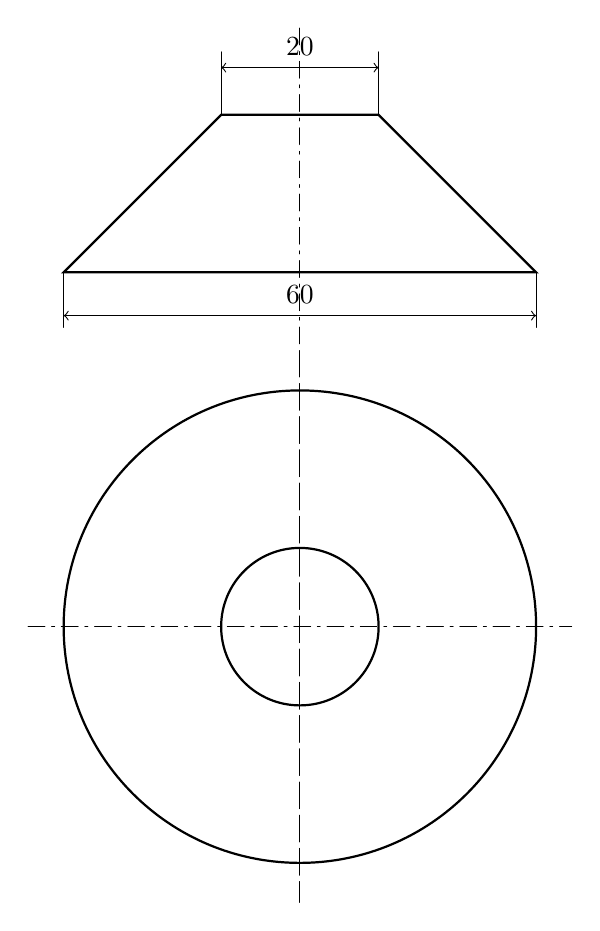
\begin{tikzpicture}[scale=0.5, line cap=round]
  % ---- 正视图：等腰梯形 ----
  \coordinate (TL) at (-2,13);
  \coordinate (TR) at (2,13);
  \coordinate (BR) at (6,9);
  \coordinate (BL) at (-6,9);
  \draw[thick] (TL)--(TR)--(BR)--(BL)--cycle;
  % 上口尺寸线 ∅20
  \draw[thin] (-2,13)--(-2,14.6);
  \draw[thin] (2,13)--(2,14.6);
  \draw[<->] (-2,14.2)--(2,14.2);
  \node[above] at (0,14.25) {$\varnothing 20$};
  % 下口尺寸线 ∅60
  \draw[thin] (-6,9)--(-6,7.6);
  \draw[thin] (6,9)--(6,7.6);
  \draw[<->] (-6,7.9)--(6,7.9);
  \node[above] at (0,7.95) {$\varnothing 60$};
  % ---- 竖直轴线（点划线，贯穿两视图）----
  \draw[dash pattern={on 6pt off 2.5pt on 1pt off 2.5pt}, thin]
        (0,15.2)--(0,-7);
  % ---- 俯视图：同心圆 ----
  \draw[thick] (0,0) circle (6);
  \draw[thick] (0,0) circle (2);
  \draw[dash pattern={on 6pt off 2.5pt on 1pt off 2.5pt}, thin]
        (-6.9,0)--(6.9,0);
  \draw[dash pattern={on 6pt off 2.5pt on 1pt off 2.5pt}, thin]
        (0,-6.9)--(0,7);
\end{tikzpicture}
\end{center}
\nopagebreak[4]
\Needspace{4\baselineskip}
\textbf{解析}

\Needspace{5\baselineskip}
正视图为等腰梯形、俯视图为同心圆，该二视图表示一个竖直放置的圆台：上底直径 $20$ 毫米、下底直径 $60$ 毫米，即

\nopagebreak[4]
\[
r_{1}=10\ \text{\text{毫米}},
\qquad
r_{2}=30\ \text{\text{毫米}}.
\]

\Needspace{5\baselineskip}
源解答按母线与底面成 $45^\circ$ 定高（两底半径之差 $r_{2}-r_{1}=20$ 毫米）：

\nopagebreak[4]
\[
h=(r_{2}-r_{1})\operatorname{tg}45^\circ=20\ \text{\text{毫米}}.
\]

\begin{gktip}
\textbf{源注}：其一，题面与二视图中均未标注任何角度，源解答径用 $45^\circ$ 定高，条件缺口由源卷自行补足，本文按源口径照录；其二，源解答代入行印作「$10^{2}+30^{2}+10\times 20$」，按圆台公式应为 $r_{1}r_{2}=10\times 30$，源解答的结果 $\dfrac{26000\pi}{3}$ 与后续方程均按 $10\times 30$ 成立，本文按 $10\times 30$ 推导。
\end{gktip}

\Needspace{5\baselineskip}
圆台体积：

\nopagebreak[4]
\[
V=\frac{\pi h}{3}\left(r_{1}^{2}+r_{2}^{2}+r_{1}r_{2}\right)
=\frac{\pi}{3}(10^{2}+30^{2}+10\times 30)\times 20
=\frac{26000\pi}{3}\ \text{\text{立方毫米}}.
\]

\Needspace{5\baselineskip}
设需截取直径 $40$ 毫米（半径 $20$ 毫米）、长 $x$ 毫米的圆柱形钢材，锻压前后体积不变：

\nopagebreak[4]
\[
\pi\cdot 20^{2}\cdot x=\frac{26000\pi}{3}
\quad\Longrightarrow\quad
x=\frac{26000}{3\times 20^{2}}=\frac{65}{3}=21\frac{2}{3}\approx 21.7\ \text{\text{毫米}}.
\]
\nopagebreak[4]
\begin{center}% 1977 年甘肃卷第六题：圆台二视图（上：正视图等腰梯形，标 ∅20、∅60；
% 下：俯视图同心圆；竖直点划线为轴线，贯穿两视图，按源卷第 3 页布局）
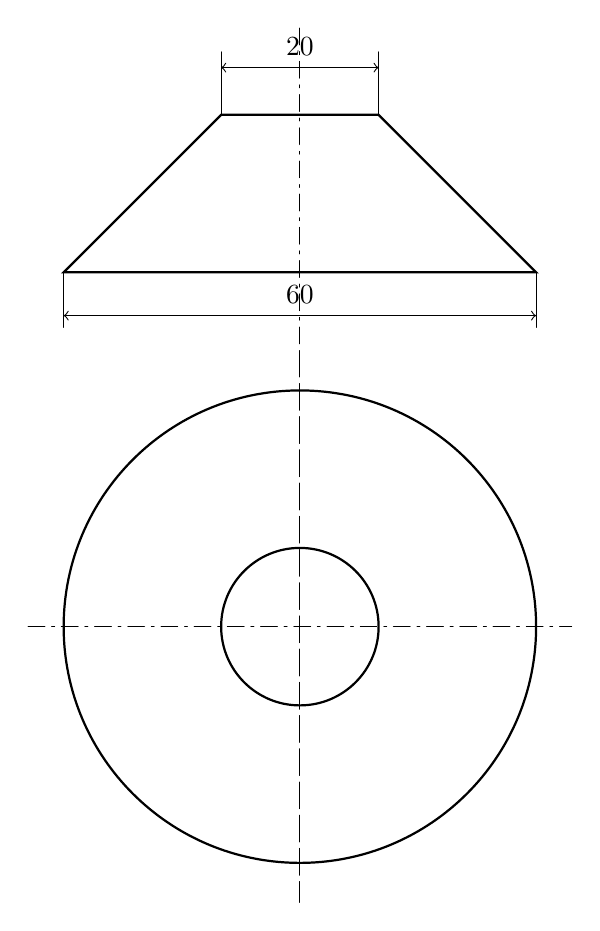
\begin{tikzpicture}[scale=0.5, line cap=round]
  % ---- 正视图：等腰梯形 ----
  \coordinate (TL) at (-2,13);
  \coordinate (TR) at (2,13);
  \coordinate (BR) at (6,9);
  \coordinate (BL) at (-6,9);
  \draw[thick] (TL)--(TR)--(BR)--(BL)--cycle;
  % 上口尺寸线 ∅20
  \draw[thin] (-2,13)--(-2,14.6);
  \draw[thin] (2,13)--(2,14.6);
  \draw[<->] (-2,14.2)--(2,14.2);
  \node[above] at (0,14.25) {$\varnothing 20$};
  % 下口尺寸线 ∅60
  \draw[thin] (-6,9)--(-6,7.6);
  \draw[thin] (6,9)--(6,7.6);
  \draw[<->] (-6,7.9)--(6,7.9);
  \node[above] at (0,7.95) {$\varnothing 60$};
  % ---- 竖直轴线（点划线，贯穿两视图）----
  \draw[dash pattern={on 6pt off 2.5pt on 1pt off 2.5pt}, thin]
        (0,15.2)--(0,-7);
  % ---- 俯视图：同心圆 ----
  \draw[thick] (0,0) circle (6);
  \draw[thick] (0,0) circle (2);
  \draw[dash pattern={on 6pt off 2.5pt on 1pt off 2.5pt}, thin]
        (-6.9,0)--(6.9,0);
  \draw[dash pattern={on 6pt off 2.5pt on 1pt off 2.5pt}, thin]
        (0,-6.9)--(0,7);
\end{tikzpicture}
\end{center}
\nopagebreak[4]
\gkanswer{答案：二视图表示圆台，体积为 $\dfrac{26000\pi}{3}$ 立方毫米；需截取直径 $40$ 毫米的圆柱形钢材 $\dfrac{65}{3}\approx 21.7$ 毫米。}

\end{answer}
\begin{answer}
\gksolhead{7}{}

\textbf{题目}：

一条直线通过 $(3,0)$，并且和直线 $y=-2x+9$ 垂直，求这条直线与直线 $2y+5x=3$ 的交点的坐标。

\Needspace{4\baselineskip}
\textbf{解析}

\Needspace{5\baselineskip}
直线 $y=-2x+9$ 的斜率为 $-2$，与它垂直的直线斜率为 $\dfrac{1}{2}$。过点 $(3,0)$、斜率 $\dfrac{1}{2}$ 的直线为

\nopagebreak[4]
\[
y-0=\frac{1}{2}(x-3),
\]

\Needspace{5\baselineskip}
即

\nopagebreak[4]
\[
x-2y=3.
\]

\Needspace{5\baselineskip}
与 $2y+5x=3$ 联立：

\nopagebreak[4]
\[
\begin{cases}
x-2y=3,\\
2y+5x=3,
\end{cases}
\]

两式相加得 $6x=6$，$x=1$；代回得 $y=-1$。故交点坐标为 $(1,-1)$。

\gkanswer{答案：交点坐标为 $(1,-1)$。}

\end{answer}
\begin{answer}
\gksolhead{8}{}

\textbf{题目}：

（1） 已知 $\dfrac{dy}{dy}=x\mathrm{e}^{x}+2\cos x+3x^2$，求 $y$；

\begin{gktip}
\textbf{源注}：源卷等式左端分母印作「$dy$」（即 $\dfrac{dy}{dy}$）；依源解答「在已知等式两边积分」的意图应为 $\dfrac{dy}{dx}$，解析正文按 $\dfrac{dy}{dx}$ 求解。
\end{gktip}

（2） 过点 $p(4,0)$ 向曲线 $x^2+y^2=1$ 作切线，求切线方程。

\Needspace{4\baselineskip}
\textbf{解析}

\gksubpart{（1）}

\Needspace{5\baselineskip}
按题面源注所记，等式实为 $\dfrac{dy}{dx}=x\mathrm{e}^{x}+2\cos x+3x^{2}$。两边对 $x$ 积分：

\nopagebreak[4]
\[
y=\int\left(x\mathrm{e}^{x}+2\cos x+3x^{2}\right)dx.
\]

\Needspace{5\baselineskip}
分项积分：$\displaystyle\int 2\cos x\,dx=2\sin x$，$\displaystyle\int 3x^{2}\,dx=x^{3}$；对 $\displaystyle\int x\mathrm{e}^{x}\,dx$ 用分部积分（取 $u=x$，$dv=\mathrm{e}^{x}dx$）：

\nopagebreak[4]
\[
\int x\mathrm{e}^{x}\,dx=x\mathrm{e}^{x}-\int \mathrm{e}^{x}\,dx=\mathrm{e}^{x}(x-1).
\]

\Needspace{5\baselineskip}
故

\nopagebreak[4]
\[
y=\mathrm{e}^{x}(x-1)+2\sin x+x^{3}+C,
\]

其中 $C$ 是任意常数。

\gksubpart{（2）}

\Needspace{5\baselineskip}
设切点为 $(x_{0},y_{0})$，圆 $x^{2}+y^{2}=1$ 在切点处的切线方程为

\nopagebreak[4]
\[
x_{0}x+y_{0}y=1.
\]

\Needspace{5\baselineskip}
因为切点在圆上，

\nopagebreak[4]
\[
x_{0}^{2}+y_{0}^{2}=1.
\]

\Needspace{5\baselineskip}
又点 $p(4,0)$ 在切线上，代入切线方程得 $4x_{0}+y_{0}\cdot 0=1$，故

\nopagebreak[4]
\[
x_{0}=\frac{1}{4},
\qquad
y_{0}=\pm\sqrt{1-x_{0}^{2}}=\pm\frac{\sqrt{15}}{4}.
\]

\Needspace{5\baselineskip}
切点为 $\left(\dfrac{1}{4},\dfrac{\sqrt{15}}{4}\right)$ 与 $\left(\dfrac{1}{4},-\dfrac{\sqrt{15}}{4}\right)$。代回切线方程并整理：

\nopagebreak[4]
\[
\frac{1}{4}x\pm\frac{\sqrt{15}}{4}y=1,
\]

\Needspace{5\baselineskip}
即所求两条切线为

\nopagebreak[4]
\[
x+\sqrt{15}\,y=4
\qquad\text{\text{与}}\qquad
x-\sqrt{15}\,y=4.
\]

\gkanswer{答案（1）：$y=\mathrm{e}^{x}(x-1)+2\sin x+x^{3}+C$（$C$ 为任意常数）。}

\gkanswer{答案（2）：$x+\sqrt{15}\,y=4$ 与 $x-\sqrt{15}\,y=4$。}

\end{answer}